\subsection{Other meshes}
In this section, some other mesh examples with irregular geometric boundaries are considered.
Fig.~\ref{qdt_ex:mesh_flower} and Fig.~\ref{qdt_ex:mesh_wolli_logo} show the mesh generated for a flower input.
Fig.~\ref{qdt_ex:mesh_flower_corners} and Fig.~\ref{qdt_ex:mesh_wolli_logo_sharp} highlight the sharp corner treatment of the algorithm.
\begin{figure}[h!]
    \begin{subfigure}[b]{1\linewidth}
        \centering
        \scalebox{0.3}{
            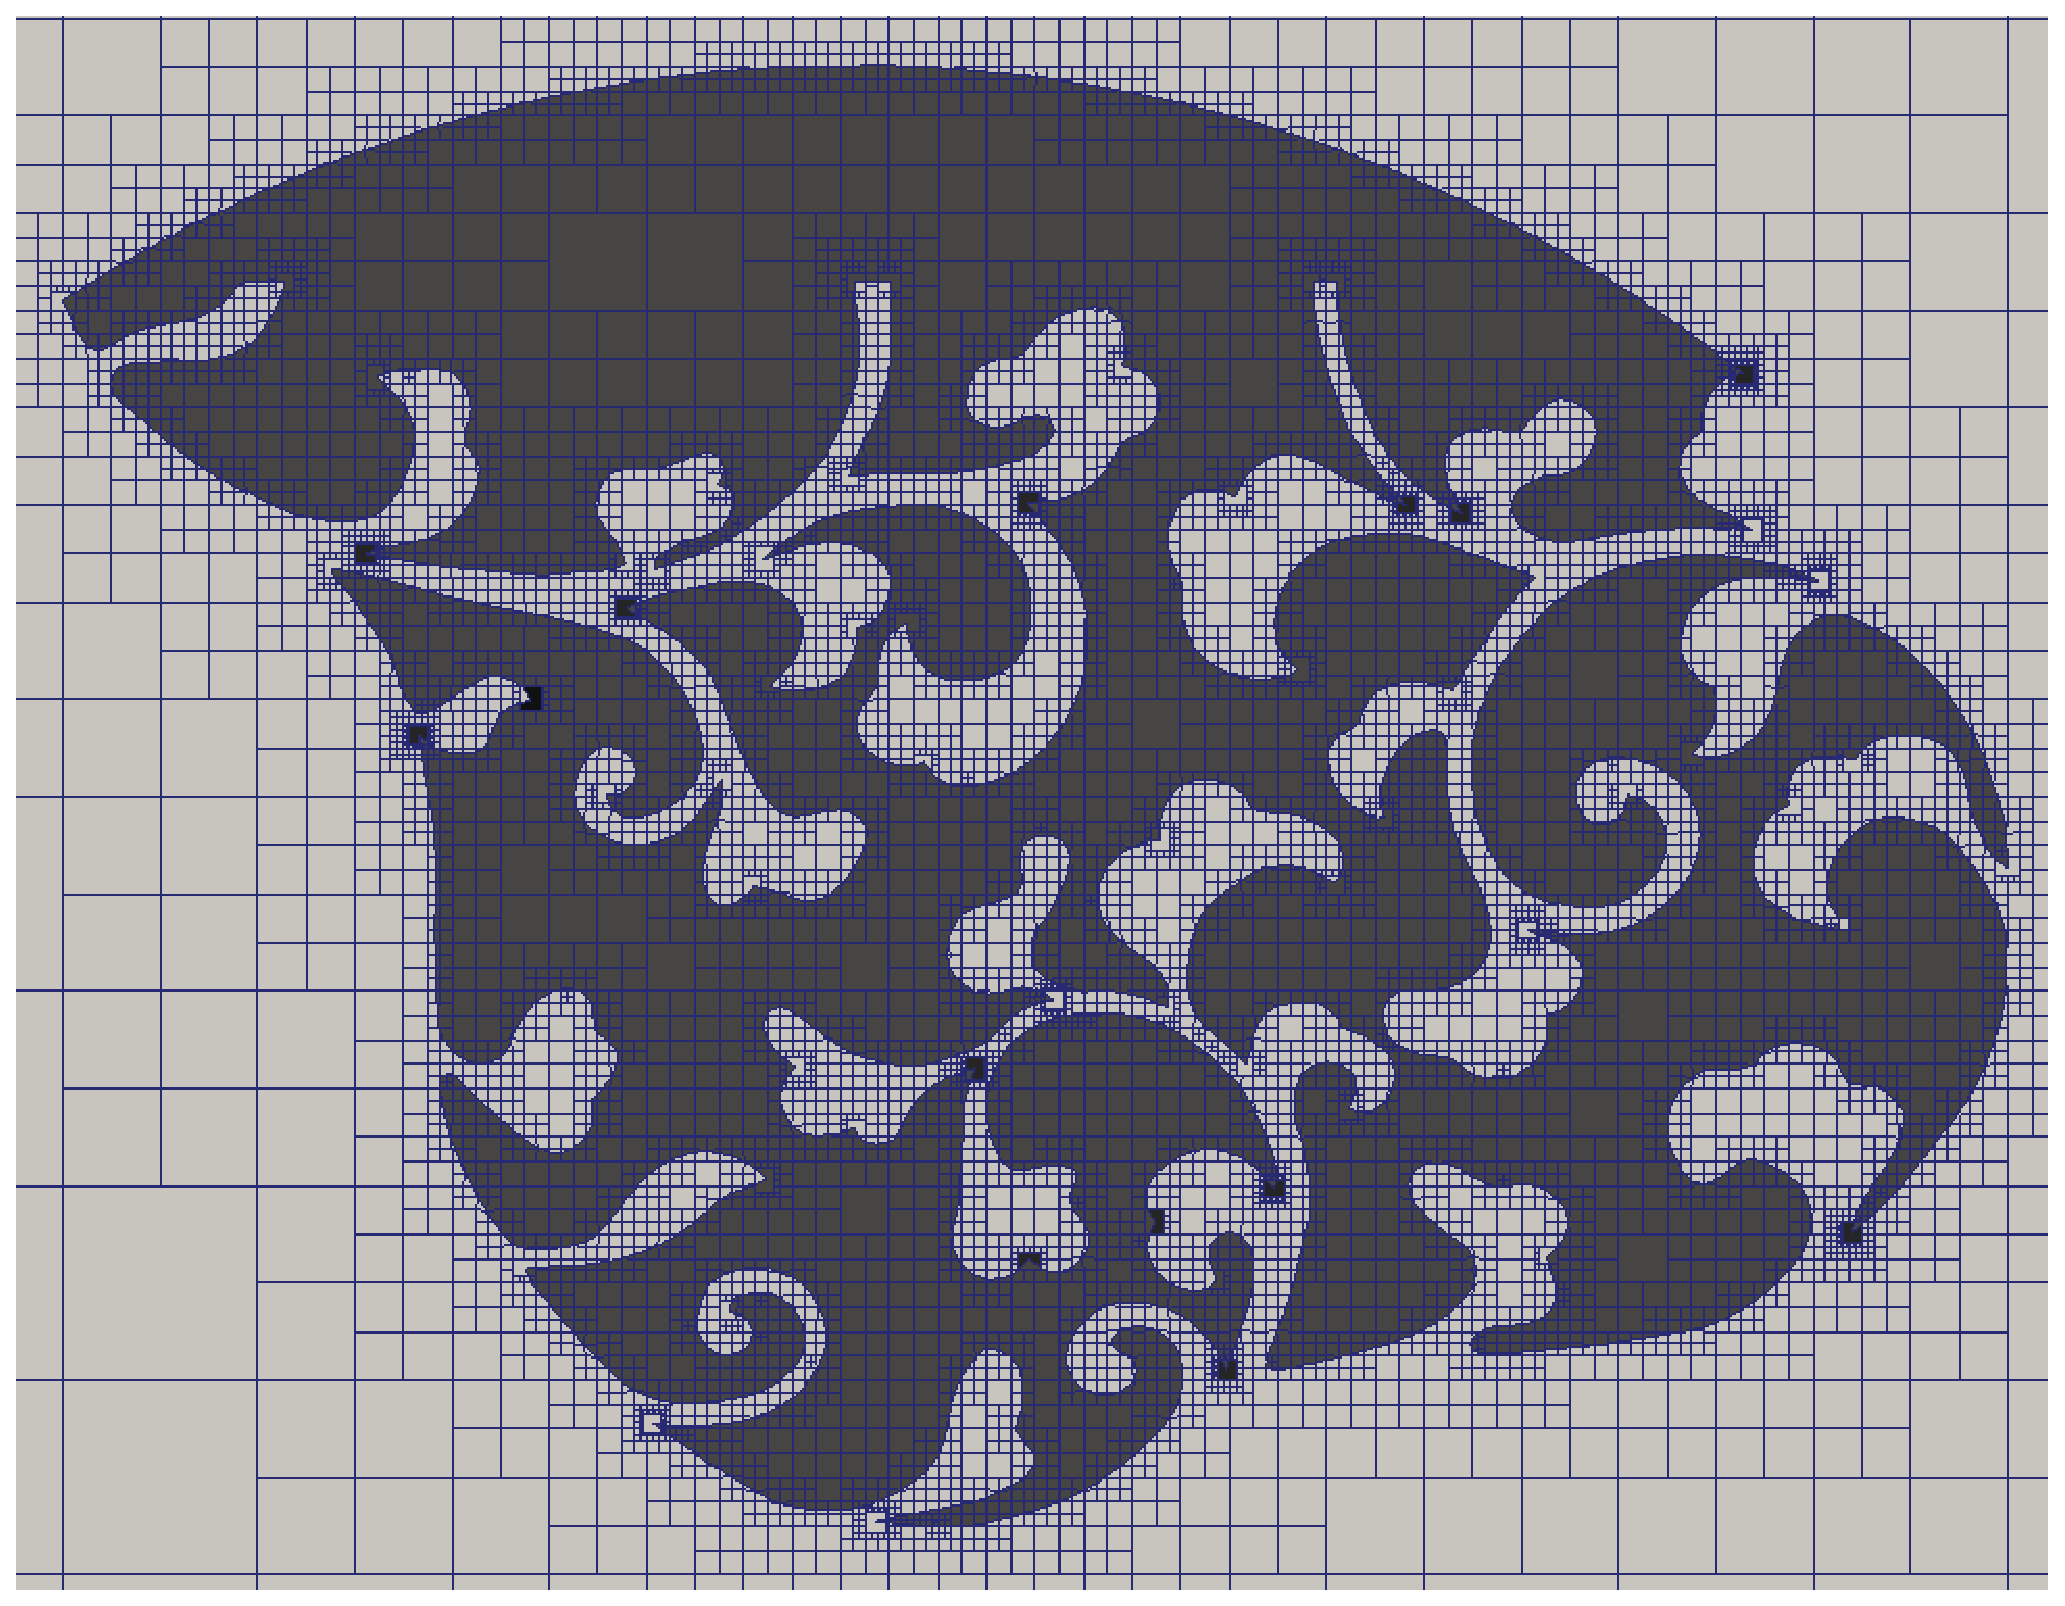
\includegraphics{quadtree/ex_images/qdt_ex_mesh_flower.eps}
        }
        \caption{Mesh for flower}
    \end{subfigure}
    \\
    \begin{subfigure}[b]{1\linewidth}
        \centering
        \scalebox{0.3}{
            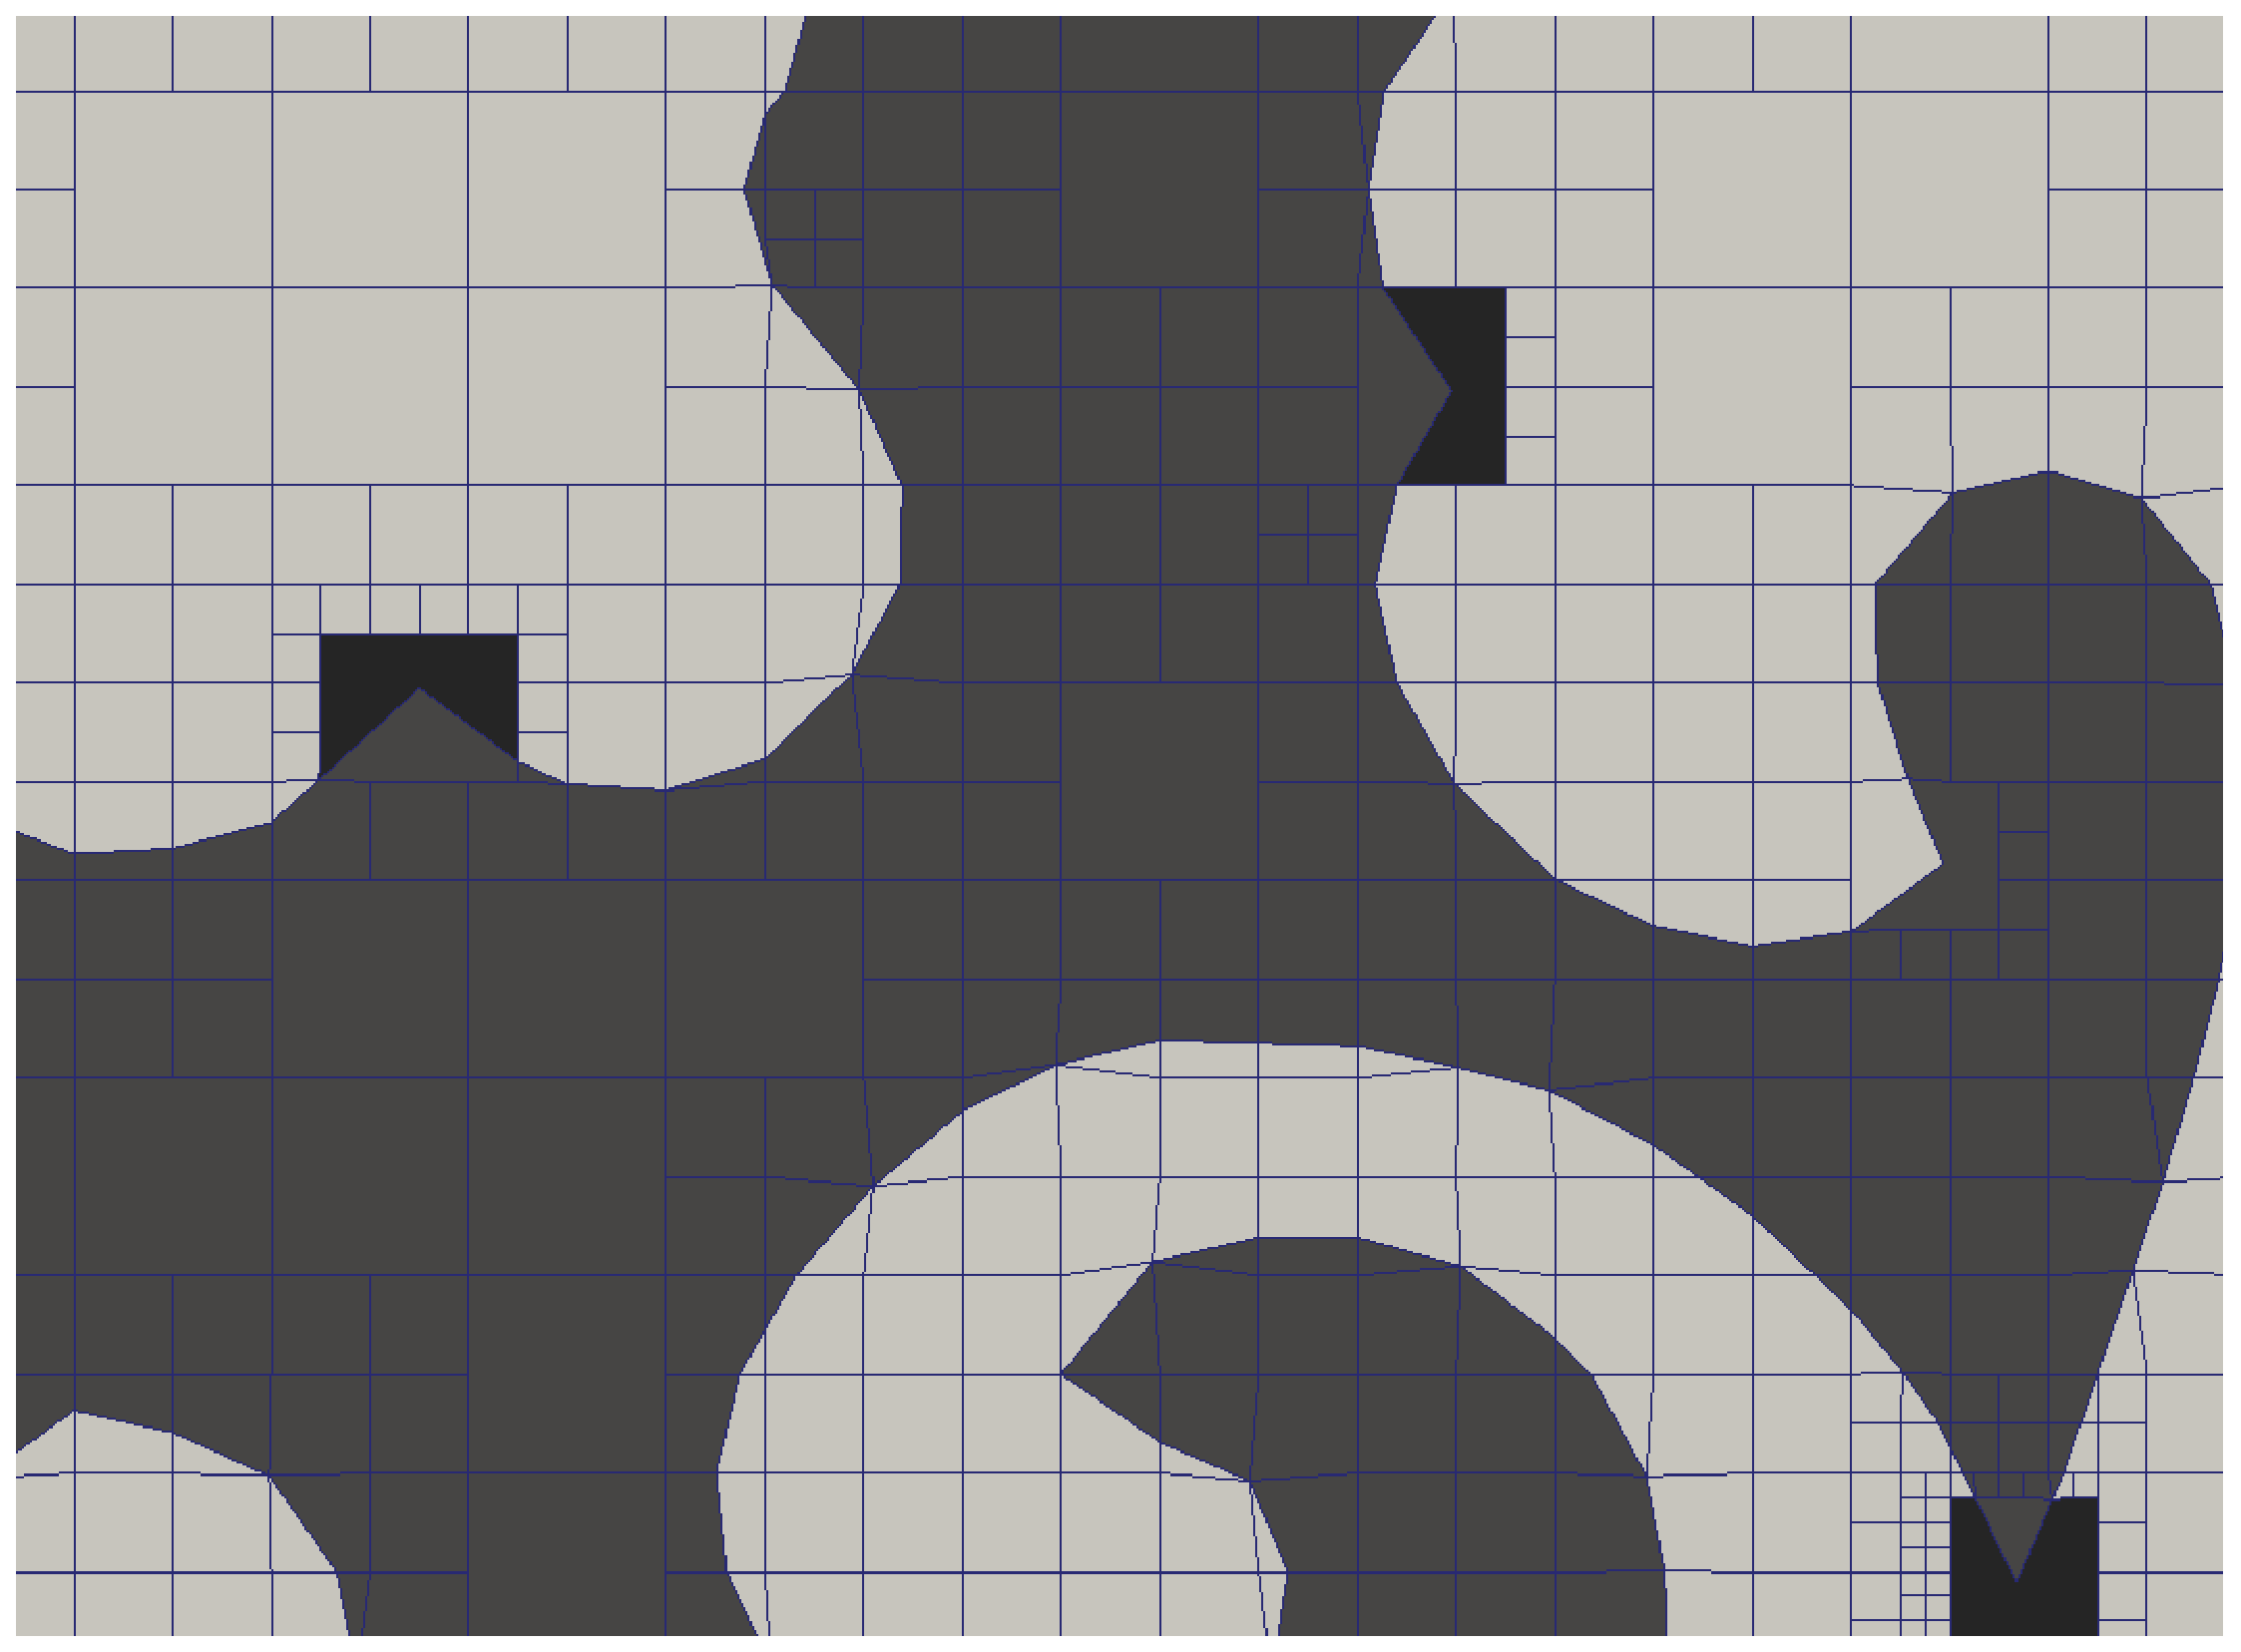
\includegraphics{quadtree/ex_images/qdt_ex_mesh_flower_sharp_corners.eps}
        }
        \caption{Mesh for flower : Sharp corners treatment}
        \label{qdt_ex:mesh_flower_corners}
    \end{subfigure}
    \caption{Mesh of flower}
    \label{qdt_ex:mesh_flower}
\end{figure}

\begin{figure}[h!]
    \begin{subfigure}[b]{1\linewidth}
        \centering
        \scalebox{0.3}{
            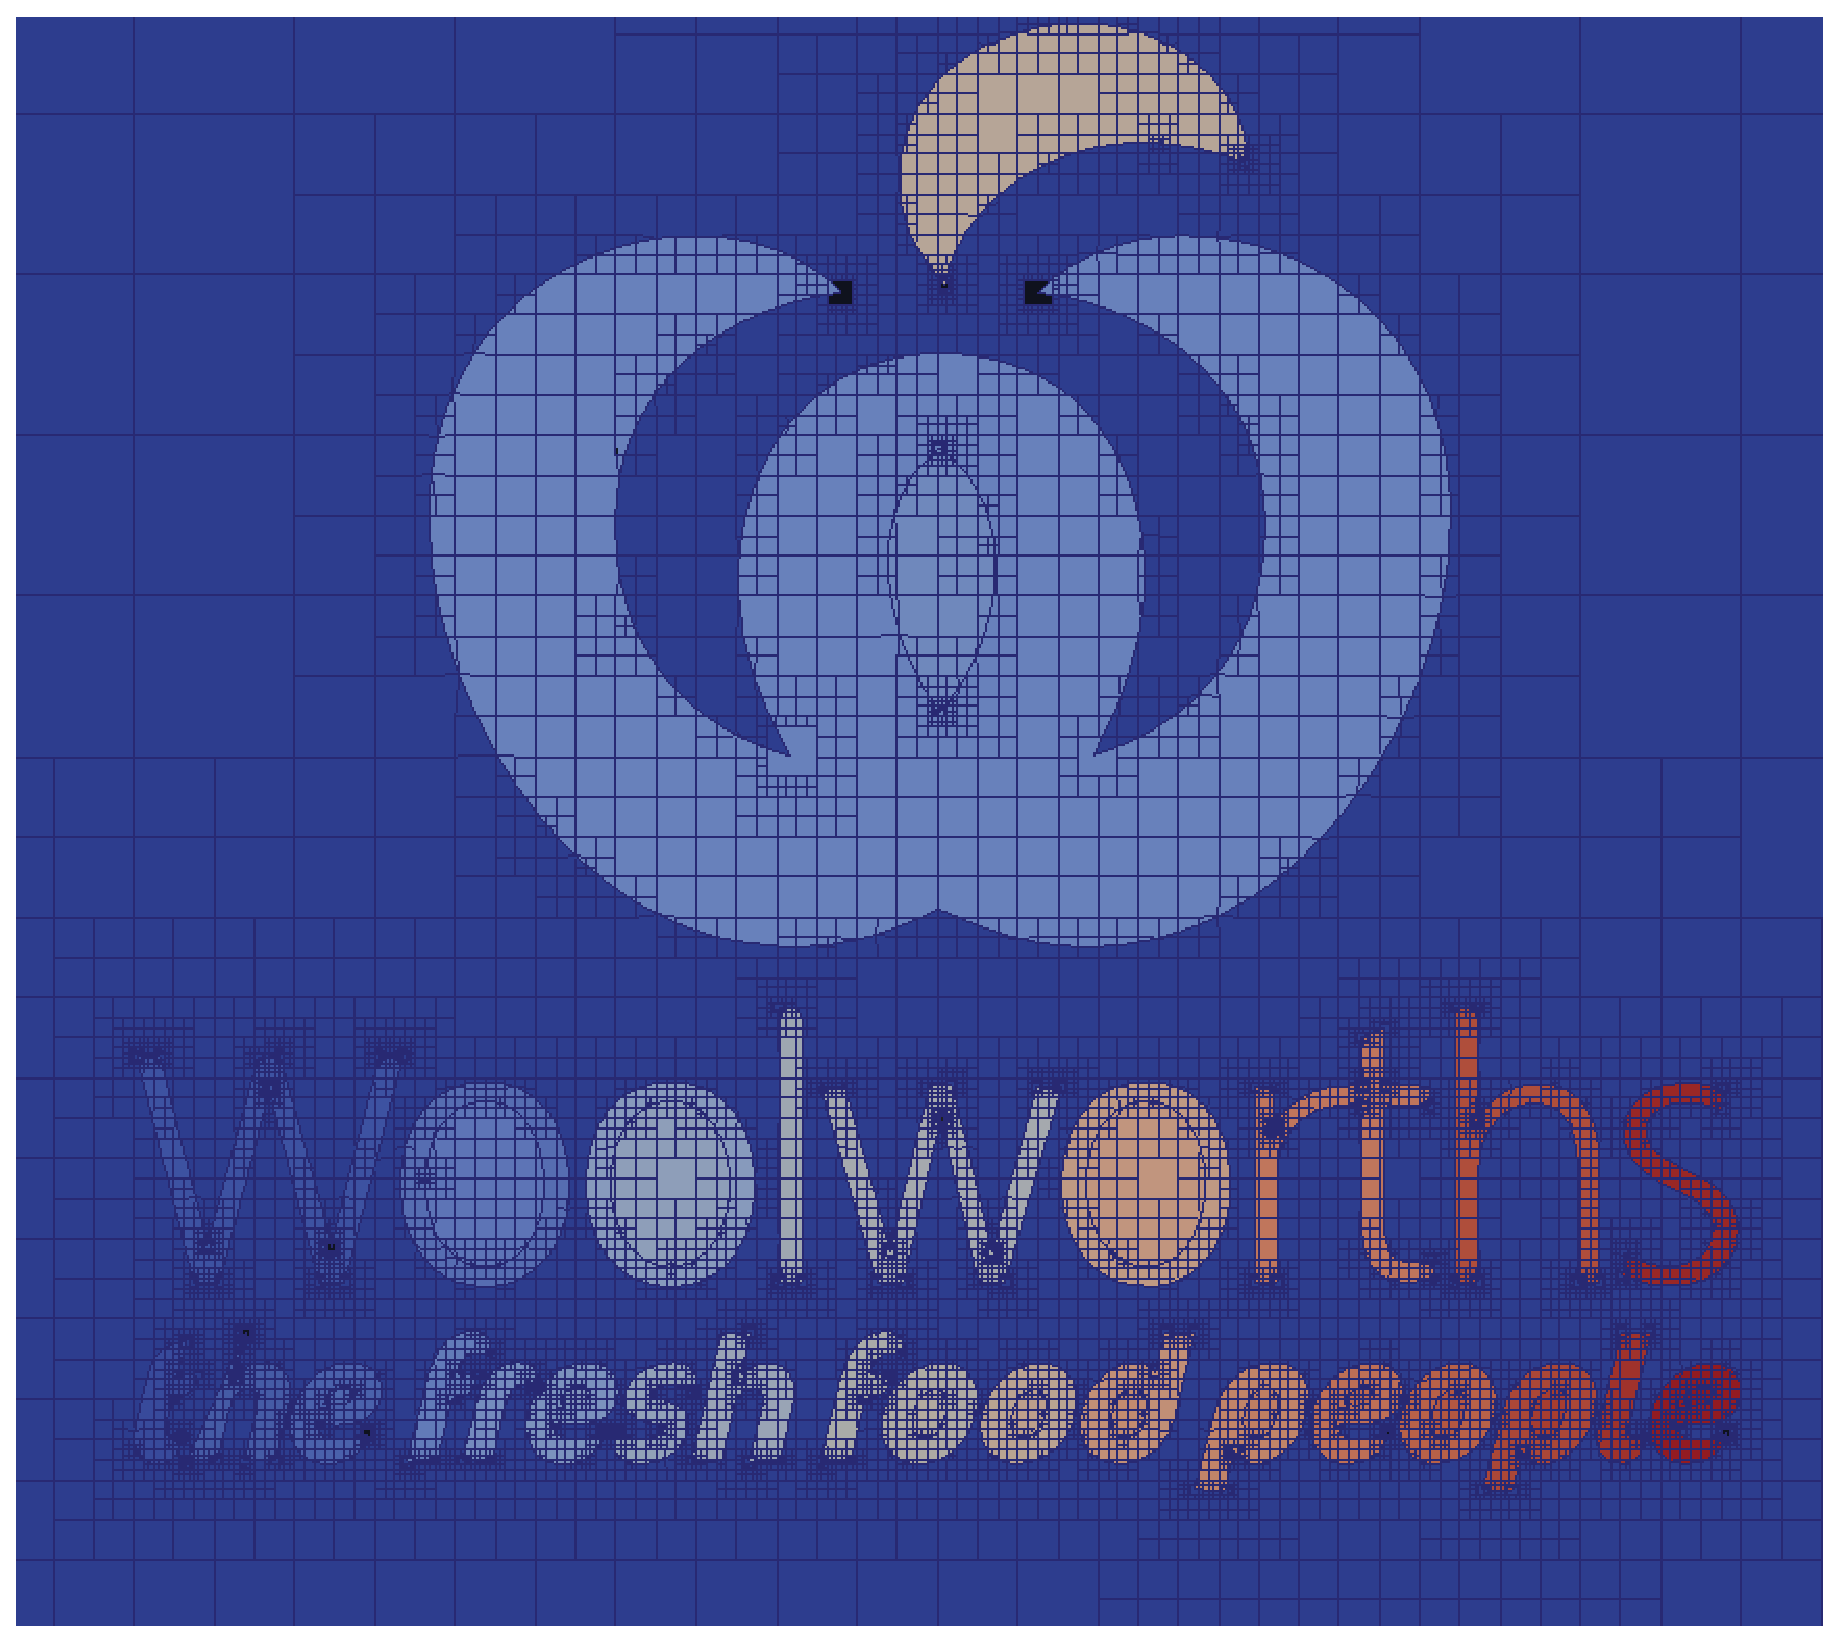
\includegraphics{quadtree/ex_images/qdt_ex_mesh_wolli.eps}
        }
        \caption{Mesh for woolworth logo : Different colors for differnet materials}
    \end{subfigure}
    \\
    \begin{subfigure}[b]{1\linewidth}
        \centering
        \scalebox{0.3}{
            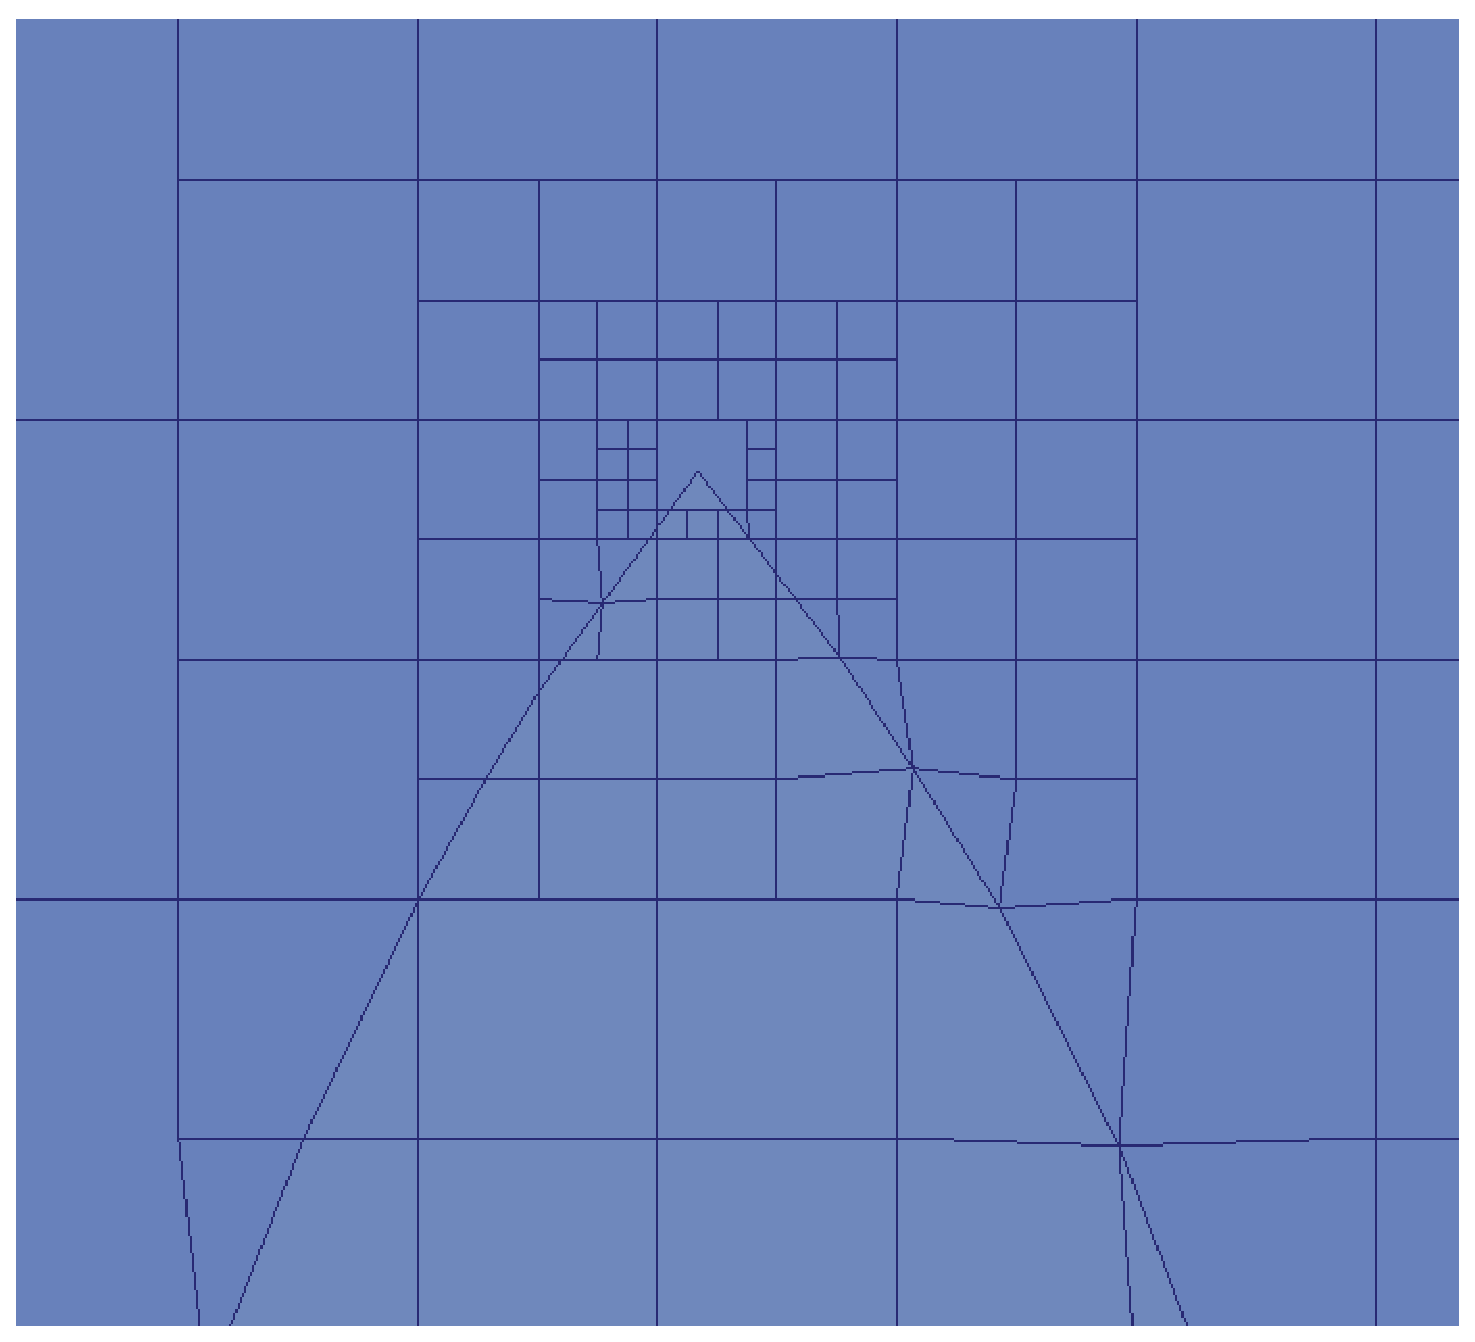
\includegraphics{quadtree/ex_images/qdt_ex_mesh_wolli_sharp_corner.eps}
        }
        \caption{Mesh for woolworth logo : Sharp conors treatment}
        \label{qdt_ex:mesh_wolli_logo_sharp}
    \end{subfigure}
    \caption{Mesh of wolli logo}
    \label{qdt_ex:mesh_wolli_logo}
\end{figure}
